\documentclass[9pt,fleqn,a4paper]{article}

\usepackage{graphicx}
\usepackage{amssymb}
\usepackage{epstopdf}
\usepackage{hyperref}
\usepackage{matlab}
\usepackage{color}
%\usepackage{sectsty}
%\allsectionsfont{\color{red}}

\DeclareGraphicsExtensions{.png,.eps,.pdf,.svg,.tiff}
\DeclareGraphicsRule{.svg}{pdf}{.pdf}{`rsvg-convert -f pdf #1 > `dirname #1`/`basename #1 .svg`-svg-converted-to.pdf}

%% FONTS

\usepackage{pifont}

\usepackage{mathptmx}
\usepackage{amsmath,amsfonts,amssymb,bm}
\setcounter{MaxMatrixCols}{20}
\usepackage[mathcal]{eucal}

\usepackage{longtable}

\usepackage{fancybox}
\usepackage{booktabs}

\usepackage{xifthen}
\newboolean{draft} 

% general layout
\setcounter{secnumdepth}{3}     % label subsubsections
\raggedbottom
%\usepackage{cite}  clashes with biblatex
\usepackage{array}
\usepackage{color}
%\usepackage{sidecap}
\usepackage[small,nooneline,bf]{caption}
%\usepackage{accents}
\setlength{\fboxsep}{0.3ex}

\ifthenelse{\boolean{draft}}{\usepackage[notref,notcite]{showkeys}} %\definecolor{refkey}{red}{1}\definecolor{labelkey}{red}{1}}
%\ifthenelse{\boolean{draft}}{\usepackage{showlabels}}

\usepackage{subfigure}

%\usepackage{appendix}   % per chapter appendices

\usepackage{endnotes}
\let\realfootnote=\footnote
\let\footnote=\endnote
%\def\enoteformat{\parindent=1.8em\leavevmode\theenmark}
%378 \def\enoteformat{\rightskip\z@ \leftskip\z@ \parindent=1.8em
%379   \leavevmode\llap{\makeenmark}}

\DeclareMathSymbol{\minus}{\mathord}{operators}{"2D}


\newcommand{\footnotex}[1]{\footnote{#1 [p. \pageref{en-\thechapter.\theenmark}]}\label{en-\thechapter.\theendnote}}

% create vertically aligned figures
%
%   \topfigure{width}{filename}
\newcommand{\centrefigure}[2]{\begin{minipage}[c]{#1}\vspace{0pt}\includegraphics[width=0.99\textwidth]{#2}\end{minipage}}
\newcommand{\topfigure}[2]{\begin{minipage}[t]{#1}\vspace{0pt}\includegraphics[width=0.99\textwidth]{#2}\end{minipage}}

%\usepackage[info]{crop}
%\crop
%\pageframetrue
%\newcommand{\topfigrule}{\hrule}

% page dimensions
%\setlength{\textwidth}{117mm}
%\setlength{\textheight}{190mm}
%\setlength{\oddsidemargin}{15mm}
%\setlength{\evensidemargin}{15mm}
%\setlength{\paperheight}{228mm}
%\setlength{\paperwidth}{150mm}

% MIT dimensions
%\setlength{\textwidth}{7in}
%\setlength{\textheight}{9in}


% paragraphs
\setlength\parindent{0pt}
\setlength{\parskip}{1ex plus 0.5ex minus 0.2ex}
\newlength\fvskip
\setlength\fvskip{0.5mm}

% figure dimensions
%
%   \figwidth   normal width for a figure
%   \figwidths  width for 2 figs side by side
%   \bigwidth   width for a figure that spans the page
\newlength{\figwidth}
\setlength{\figwidth}{0.6\textwidth}
\newlength{\figwidths}
\setlength{\figwidths}{0.45\textwidth}
\newlength{\bigwidth}		% for root-locus plots
\setlength{\bigwidth}{\textwidth}
\newlength{\fullwidth}
\setlength{\fullwidth}{\textwidth}

% headers and footers
\usepackage{fancyheadings}
%\pagestyle{headings}
\pagestyle{fancy}
\addtolength{\headheight}{4pt}
%%\addtolength{\headwidth}{\marginparsep}
%%\addtolength{\headwidth}{\marginparwidth}
%%%\renewcommand{\chaptermark}[1]{\markboth{#1}{#1}} % remember chapter title
%%%\renewcommand{\sectionmark}[1]{\markright{\thesection\ #1}}
                                              % section number and title
\lhead[\fancyplain{}{\bf\thepage}]{\fancyplain{}{\bf\rightmark}}
\rhead[\fancyplain{}{\bf\leftmark}]{\fancyplain{}{\bf\thepage}}
\cfoot{}
%\lfoot{Draft of \today, Boston}
%\lfoot{Draft of \today, Brisbane}
\lfoot{Draft of \today, Brisbane}
\rfoot{Copyright (c) Peter Corke 2015}
\def\fps@figure{htp}
\def\fps@table{htp}

% hypenation rules
\hyphenation{ro-botic}
\hyphenation{ro-botics}

% float placement
\def\topfraction{.9}
\def\bottomfraction{.9}
\def\textfraction{.1}
\def\floatpagefraction{.9}
%\renewcommand{\caption}{\hangcaption}
%
%\def\figurestring{figure}



%%%%%%%%%%%%%%%%%%%%%%%%%%%%%%%%%%%%%%%%%%%%%%%%%%%%%%%
%        extra packages
%%%%%%%%%%%%%%%%%%%%%%%%%%%%%%%%%%%%%%%%%%%%%%%%%%%%%%%

% create the strikeout macro
\usepackage{ulem}
\normalem

%\usepackage[hyphens]{url}

\usepackage{marginnote}
\newcommand{\todo}[1]{\ifthenelse{\boolean{draft}}{\marginnote{{\color{red}#1}}}{}}

%\usepackage{wrapfig}

% Info box environment
%   for detailed information about Toolbox functions
%
%   \begin{InfoBox}
%   \end{InfoBox}
\usepackage{float}

\definecolor{Yellow}{rgb}{1, 1, 0.8}
%\definecolor{Yellow}{rgb}{1, 1, 0.9}
\definecolor{Blue}{rgb}{0.9, 0.9, 1} % sky blue
\definecolor{Red}{rgb}{1, 0.7, 0.7}


\newcommand{\advise}[1]{{\color{red}#1}}
\makeatletter\newenvironment{BlueBox}%
   {\begin{lrbox}{\@tempboxa}\begin{minipage}{\columnwidth}}%
   {\end{minipage}\end{lrbox}%
      \colorbox{Blue}{\usebox{\@tempboxa}}
      }\makeatother

\makeatletter\newenvironment{YellowBox}%
   {\begin{lrbox}{\@tempboxa}\begin{minipage}{\columnwidth}}%
   {\end{minipage}\end{lrbox}%
      \colorbox{Yellow}{\usebox{\@tempboxa}}
      }\makeatother

\makeatletter\newenvironment{InfoBox}%
   {\begin{lrbox}{\@tempboxa}\begin{minipage}{\columnwidth}}%
   {\end{minipage}\end{lrbox}%
      \colorbox{Blue}{\usebox{\@tempboxa}}
      }\makeatother

\makeatletter\newenvironment{WarningBox}%
   {\begin{lrbox}{\@tempboxa}\begin{minipage}{\columnwidth}}%
   {\end{minipage}\end{lrbox}%
      \colorbox{Red}{\usebox{\@tempboxa}}
      }\makeatother

% \begin{BioAside}{image}{firstname}{lastname}{years}

\floatstyle{plain}
\newfloat{AsideFloat}{b}{loi}[section]
\newenvironment{Aside}{\begin{AsideFloat}\begin{BlueBox}\footnotesize}{\end{BlueBox}\end{AsideFloat}}
\newenvironment{AsideNoFloat}{\begin{BlueBox}\footnotesize}{\end{BlueBox}}

%\newenvironment{BioAside}[4]{\begin{AsideFloat}\begin{BlueBox}\footnotesize    \begin{tabular}{lp{90mm}}\begin{minipage}[t]{2cm}\vspace{0pt}\includegraphics[width=2cm]{figs/people/#1}\end{minipage}&\textbf{#2 #3 (#4)}\index{people}{#3, #2|textbf}}{\end{tabular}\end{BlueBox}\end{AsideFloat}}
% \begin{BioAside}{fig}{first}{second}{years}
\newenvironment{BioAside}[4]{\begin{PicAside}[20mm]{#1}\textbf{#2 #3 (#4)}\index{people}{#3, #2|textbf}}{\end{PicAside}}
\newenvironment{BioAsideNoPic}[3]{\begin{AsideFloat}\begin{YellowBox}\footnotesize \textbf{#1 #2 (#3)}\index{people}{#2, #1|textbf}}{\end{YellowBox}\end{AsideFloat}}

% begin{PicAside}{image}{lines}
% begin{PicAside}[width]{image}{lines}
%  lines is number of lines of text for the wrapped figure, if empty {} then computed

%\newenvironment{PicAside}[2][20mm]{\begin{AsideFloat}\begin{BlueBox}\footnotesize    \begin{tabular}{lp{110mm-#1}}\begin{minipage}[t]{#1}\vspace{0pt}\includegraphics[width=#1]{#2}\end{minipage}&}{\end{tabular}\end{BlueBox}\end{AsideFloat}}
\newenvironment{PicAside}[2][20mm]{%
\begin{AsideFloat}\begin{minipage}{#1}\vspace{0pt}\includegraphics[width=#1]{#2}\end{minipage}\hspace{1ex}%
\begin{minipage}[t]{110mm-#1}\begin{BlueBox}\footnotesize}%
{\end{BlueBox}\end{minipage}\end{AsideFloat}}
\newenvironment{PicAsideNoFloat}[2][20mm]{%
\begin{minipage}{#1}\vspace{0pt}\includegraphics[width=#1]{#2}\end{minipage}\hspace{1ex}%
\begin{minipage}[t]{110mm-#1}\begin{BlueBox}\footnotesize}%
{\end{BlueBox}\end{minipage}}

% begin{PicWrapAside}{image}{lines]
% begin{PicWrapAside}[width]{image}
\newenvironment{PicWrapAside}[3][20mm]{\begin{AsideFloat}\begin{YellowBox}\footnotesize\begin{minipage}[t]{\textwidth}\begin{wrapfigure}[#3]{l}{#1}
\includegraphics[width=#1]{#2}
\end{wrapfigure}}
{\end{minipage}\end{YellowBox}\end{AsideFloat}}

\floatstyle{boxed}
%\newfloat{Info}{b}{loi}[chapter]
%\newenvironment{InfoBox}{\begin{Info}\footnotesize}{\end{Info}}

%\newcolumntype{V}{>{\centering\arraybackslash} m{.4\linewidth} }


% Biography box environment
%   for information about people or organizations.
%
%   \begin{BioBox}
%   \end{BioBox}
\floatstyle{boxed}
%\newfloat{Biography}{b}{lob}[chapter]
\newenvironment{BioBox}{\begin{Biography}\footnotesize}{\end{Biography}}

% Matlab code example environment
%   for code examples.
%   each executable line must begin with >>
%   comments start with !
%   lines starting !>> are executed during parsing, but dont print
%   
%   \begin{Code}
%   \end{Code}

%\definecolor{orange}{rgb}{0.5,0.28,0}
\definecolor{orange}{rgb}{1,0,0}
\definecolor{grey}{rgb}{0.5,0.5,0.5}
  
\usepackage{fancyvrb}
\fvset{formatcom=\color{orange},fontseries=c,fontfamily=courier,xleftmargin=4mm,commentchar=!}

\DefineVerbatimEnvironment{Code}{Verbatim}{formatcom=\color{blue},fontseries=c,fontfamily=courier,fontsize=\footnotesize,commentchar=@,xleftmargin=4mm,commandchars=\\\{\}}
\DefineVerbatimEnvironment{CodeGrey}{Verbatim}{formatcom=\color{grey},fontseries=c,fontfamily=courier,fontsize=\footnotesize,commentchar=@,xleftmargin=4mm,commandchars=\\\{\}}

\DefineVerbatimEnvironment{CodeSmall}{Verbatim}{formatcom=\color{blue},fontseries=c,fontfamily=courier,fontsize=\scriptsize,xleftmargin=1mm,commentchar=!}

\DefineVerbatimEnvironment{XML}{Verbatim}{formatcom=\color{orange},fontseries=c,fontfamily=courier,fontsize=\footnotesize,commentchar=@,xleftmargin=4mm,commandchars=\\\{\}}
\DefineVerbatimEnvironment{XMLNum}{Verbatim}{numbers=left,numbersep=4pt,formatcom=\color{orange},fontseries=c,fontfamily=courier,fontsize=\footnotesize,xleftmargin=4mm}

\newcommand{\xml}[1]{{\color{orange}\Verb+#1+}}

%\makeatletter\newenvironment{Code}%
%   {\begin{Verbatim}[formatcom=\color{blue},fontseries=c,fontfamily=courier,fontsize=\footnotesize,xleftmargin=4mm,commentchar=!]}%
%   {\end{Verbatim}\vspace{-0.8ex}}\makeatother
%

\DefineVerbatimEnvironment{CodeNoParse}{Verbatim}{formatcom=\color{blue},fontseries=c,fontfamily=courier,fontsize=\footnotesize,xleftmargin=4mm,commentchar=!}
\DefineVerbatimEnvironment{CodeNum}{Verbatim}{numbers=left,numbersep=4pt,formatcom=\color{blue},fontseries=c,fontfamily=courier,fontsize=\footnotesize,xleftmargin=4mm}


% future work, can we put code segment numbers in the margin?
\newcounter{example}
\setcounter{example}{1}
%\newenvironment{Example}{\marginnote{\vspace{12pt}\color{blue}Ex \thechapter.\theexample}\addtocounter{example}\DefineShortVerb{\|}\SaveVerb{Verb}|}{|\UseVerb{Verb}}
%\newenvironment{Example}{\DefineShortVerb{\|}\SaveVerb{Verb}|}{|\UseVerb{Verb}}
%\newcommand{\fvmarginnote}{\marginnote{\vspace{12pt}\color{blue}Ex \thechapter.\theexample}\addtocounter{example}}
%\newcommand{\fvmarginnote}{\marginnote{Ex \thechapter.\theexample}\addtocounter{example}{1}}
\newcommand{\fvmarginnote}{}
\def\exlabel#1{{\string\newlabel{#1}{{Bob}{\thepage}}}}

\usepackage{empheq}
\definecolor{eqboxcolor}{rgb}{0.9608,    0.9608,    0.8627}
\newcommand*\eqbox[1]{%
 \colorbox{eqboxcolor}{\hspace{1em}#1\hspace{1em}}}
%\usepackage{mybib}

\usepackage{marginnote}
\newcommand{\sidenote}[1]{~$\blacktriangleright$\marginnote{\tiny #1}}
\usepackage{framed}


\typeout{------ end of layout ------}

\include{notation}


\lfoot{}
\rfoot{}


%\usepackage{upquote}

%\usepackage[marginparsep=5mm]{marginnote}
\usepackage{marginnote}
\usepackage{url}

\title{Understanding URDF using MATLAB\textsuperscript{\textregistered}}
\author{Peter Corke}
\date{November 2018}                                           % Activate to display a given date or no date

\begin{document}
\maketitle

\section{Introduction}
The Universal Robot Data Format (URDF) is an increasingly common way to represent the kinematic structure and visual appearance of robots.
It is widely used in the ROS software ecosystem.
A URDF file is an XML format file and a number of specialized tags.

I've not found a particularly helpful or readable tutorial hence I'm writing my own.

\section{XML 101}
URDF files are expressed in XML so it's helpful to start with a refresher about XML.

\subsection{What's in an XML file}
The most obvious feature of an XML document are the angle-bracket-delimited \emph{tags}  such as \xml{<foo>} or \xml{<bar>}.
The file contains structured text that can be read by a person as well as being easy to parse programatically.

An XML file is frequently referred to as a \textit{document}.
The file comprises \emph{markup} and \emph{content}.
Generally, strings that constitute markup either begin with the character \xml{<} and end with a \xml{>}, or they begin with the character \xml{\&} and end with a \xml{;}. Strings of characters that are not markup are content.

\subsubsection{Tags}

A \emph{tag} is a markup construct that begins with \xml{<} and ends with \xml{>}. Tags come in three flavours:
\begin{description}
\item[start-tag] such as \xml{<tag>}
\item[end-tag] such as \xml{</tag>}
\item[empty-element tag] such as \xml{<tag />}
\end{description}
where, in all cases, \xml{tag} is the name of the tag and is given without quotes.  For example \xml{<foo>} is a tag named foo.
Tag names start with a letter, underscore or colon, followed by alphanumeric, dot or underscore characters.  

\subsubsection{Elements}
An \emph{element} is a logical document component that either begins with a start-tag and ends with a matching end-tag or consists only of an empty-element tag. The characters between the start-tag and end-tag, if any, are the element's \emph{content}, and may contain markup, including other elements, which are called child elements. 

An XML element has matching start and end tags like
\begin{XML}
<foo></foo>
\end{XML}
or single empty-element tag such as
\begin{XML} 
<bar />
\end{XML}
which is equivalent to 
\begin{XML} 
<bar></bar>
\end{XML}

The body of the \textit{element} can be an arbitrary mixture of plain text or other elements, ie. elements can be nested within the body of
other elements.  This allows the creation of hierarchies or trees, with the first or outermost element as the root.
For example:
\begin{XML}
<bar>some text</bar>
<foo><bar>one</bar><bar>two</bar></foo>
\end{XML}

The elements must not overlap. i.e., an end tag of an element must have the same name as that of the most recent unmatched start tag.

\subsubsection{Attributes}

An \emph{attribute} is a markup construct consisting of \xml{name=value} pairs that exists within a start-tag or empty-element tag. 
The \textit{attributes} are given as a name and a value.
Attribute names are defined without quotation marks, whereas attribute values must always appear as a string delimited with either single or double quotes.
For example
\begin{quote}
 \xml{<img src="madonna.jpg" alt="Madonna" />}
\end{quote}
has two \emph{attributes}.  Their names are \xml{"src"} and \xml{"alt"}, and their \emph{values} are \xml{"madonna.jpg"} and \xml{"Madonna"} respectively.  
An XML attribute can only have a single value and each attribute can appear at most once on each element.
Attribute names start with a letter, underscore or colon, followed by alphanumeric, dot or underscore characters.  
Attribute names in XML (unlike HTML) are case sensitive. 

\subsubsection{Special characters \&$\cdot\cdot$;}
Special characters are introduced using XML references.
References always begin with the symbol \xml{"\&"} which is a reserved character and end with the symbol \xml{";"}. XML has two types of references
\begin{description}

\item[Entity References] contain a name between the start and the end delimiters.  The name refers to a predefined strings such as 

\begin{tabular}{ll}
\xml{\&amp;} & ampersand \\
\xml{\&apos;} &single quote\\
 \xml{\&gt;} & greater than\\
\xml{\&lt;} & less than \\
\xml{\&quot;} & double quote 
\end{tabular}

or a larger set defined for HTML which can be found in \href{https://en.wikipedia.org/wiki/List_of_XML_and_HTML_character_entity_references#Standard_public_entity_sets_for_characters}{online lists},
for example, \xml{\&theta;} is the Greek letter $\theta$.

\item[Character References] These specify a character by its Unicode code in either decimal or hexadecimal format.
For example the Roman character ``A'' can be specified as  \xml{\&\#65;} in decimal or \xml{\&\#x41;} in hexadecimal.
\end{description}

Because ampersand \xml{"\&"} indicates a reference it must always be escaped in text as \xml{\&amp;}.

\subsubsection{Comments and white space}

Comments are a special kind of element
\begin{XML}
<!-- comment stuff -->
\end{XML}
and the body of the comment can also span multiple lines
\begin{XML}
<!--   comment
       more comment
       still more comment -->
\end{XML}
Comments cannot be nested.

White space is mostly insignificant so XML files are often formatted with indenting to highlight the structure to human readers.  Some
editors support auto-indenting.

White space is ignored outside of quotes, so the following two lines are equivalent
\begin{XML}
\xml{<foo param1 = "x1" param2 = "x2"> body </tag>}
<foo param1="x1" param2="x2"> body </tag>
\end{XML}

\subsubsection{CDATA}
A CDATA block refers to character data that is considered literally. The special characters are interpreted as themselves, and \textit{not} as markup. 
For example
\begin{XML}
<![CDATA[
   characters with markup like 3<4;
]]>
\end{XML}
This section may contain markup characters (\xml{<}, \xml{>}, and \xml{\&}).  CDATA cannot contain the string \xml{"]]>"}.
This is somewhat analogous to a LaTeX verbatim block.


\subsubsection{Document}
XML documents may begin with an XML declaration that describes some information about themselves. An example is 
\begin{XML}
<?xml version="1.0" encoding="UTF-8"?>
\end{XML}
which is case-sensitive and must be the first statement in the document.
An XML document can have only one root element. 

\subsection{The DOM model}
The Document Object Model (DOM) is a hierarchical or tree representation of the file called a node tree.
Everything in an XML document is a node:
\begin{itemize}
\item The entire document is a document node
\item Every XML element is an element node
\item The non-markup text in the XML elements are text nodes
\item Every attribute is an attribute node
\item Comments are comment nodes
\end{itemize}
The document node is the root of the tree.  If must have at most one (XML rule) child node.  That node may have multiple children of the types mentioned above.
For example the XML element \xml{<date type="year">2005</date>} is represented by an element node \xml{<date>} with two child nodes:
an attribute node with the name \xml{"type"} and value \xml{"year"}, and a child text node with the value \xml{"2005"}.

\subsection{Reading XML with MATLAB}
Consider a short XML file that represents employees at a company
\begin{XMLNum}
<?xml version="1.0"?>
<people>

  <person employee_number="123" gender="female" >
    <name>Alice</name>
    <address>11 Alice St</address>
    <commenced date="2016-01-01" />
  </person>

  < person employee_number =  "237" gender = "male" status="on vacation" >
    <name>Bob</name>
    <commenced date="2015-07-07" />
    <address>13  Bob St</address>
  </person>

</people>
\end{XMLNum}


MATLAB provides a function to read and parse an XML file and return a DOM node-tree
\begin{Code}
>> root = xmlread('simple.xml');
\end{Code}
The type of a node is indicated by an enum  
\begin{Code}
root.getNodeType()
ans =
    9
\end{Code}
which Table \ref{tab:values} indicates is a document node.
The Table also shows the \emph{name} and \emph{value} associated with different types of node.
These are the display value of the variable, shown when it is evaluated without  a semicolon on the end of the line
\begin{Code}
>> root
root =
[#document: null]
\end{Code}

\begin{table}
\begin{tabular}{|l|l|l|l|} \hline
Node type & nodeName() & nodeType() & nodeValue()  \\ \hline\hline
Element  & tag name & ELEMENT\_NODE = 1  & null\\
Attribute  & attribute name & ATTRIBUTE\_NODE =2 &  attribute value\\
Text  & \#text & TEXT\_NODE = 3  & the string \\
CDATA  &  \#cdata-section & CDATA\_SECTION\_NODE=4  & the CDATA text \\
Entity  & entity name & ENTITY\_NODE=6  & null \\
Comment  & \#comment & COMMENT\_NODE=8  & the comment\\
Document  & \#document & DOCUMENT\_NODE=9  & null\\ \hline
\end{tabular}
\caption{Names and values for different node types.  The symbolic value in column 3 is a property of any node, ie. \texttt{node.ATTRIBUTE\_NODE} is the value 2.}\label{tab:values}
\end{table}

This root node has at least one child node
\begin{Code}
>> root.hasChildNodes
ans =  logical
   1
\end{Code}
and we can get a list of the child nodes
\begin{Code}
>> rootChildNodes = root.getChildNodes;
>> rootChildNodes.getLength
ans =
     1
\end{Code}
The first (and only) child node from this list is
\begin{Code}
>> node = rootChildNodes.item(0)
ans =
[people: null]
>> node.getNodeType
ans =
     1
\end{Code}
which is an element node and the display value shows the tag name: people.

The syntax looks quite unMATLAB-like and that's because the implementation is based on the standard Java DOM processor and the objects are native Java objects.  Elements in the list are indexed starting at zero, and we use properties and methods of the Java objects.

This node has a name, the tag name, but no value
\begin{Code}
>> node.getNodeName
ans =
people

>> node.getNodeValue
ans =
     []
\end{Code}

The people node has five children
\begin{Code}
>> persons = node.getChildNodes();
>> persons.getLength()
ans =
     5
\end{Code}
which is somewhat surprising since the people node has only two children, the two person nodes: Alice and Bob.
We can list the child nodes
\begin{Code}
>> for i=0:node.getLength-1
   persons.item(i)
 end

ans =
[#text: 

    ]

ans =
[person: null]

ans =
[#text: 

    ]

ans =
[person: null]

ans =
[#text: 

]
\end{Code}
and what we've overlooked is the non-markup text in the XML file, the three blank lines.
Since we are only interested in the \xml{person} nodes we can extract them specifically\footnote{The \texttt{getElementsByTagName} method
returns all nodes with the matching tag below \texttt{node} in the parse tree.  There is no way to restrict this to immediate children, to do that you need to find all the children and test if they have this tag.}
\begin{Code}
>> persons = node.getElementsByTagName('person');
>> persons.getLength
ans =
     2
\end{Code}   
The first person is 
\begin{Code}
>> person = persons.item(0)
person =
[person: null]
>> nodes = person.getChildNodes;
>> nodes.getLength
ans =
     7
\end{Code} 
which has seven child nodes.
Once again, we see that this is due to white space in the file
\begin{Code}
>> for i=0:nodes.getLength-1
    nodes.item(i)
end

ans =
[#text: 
      ]

ans =
[name: null]

ans =
[#text: 
      ]

ans =
[address: null]

ans =
[#text: 
      ]

ans =
[commenced: null]

ans =
[#text: 
    ]
\end{Code}
The address node could be obtained by
\begin{Code}
>> address = nodes.item(3)
address =
[address: null]
\end{Code}
but the index could vary depending on the formatting (white space) in the XML file.  It can be obtained more robustly by
\begin{Code}
>> address = nodes.getElementsByTagName('address').item(0)
address =
[address: null]
\end{Code}
noting that the \texttt{.item(0)} is required because the \texttt{getElementsByTagName} method always returns a list.
The address node has just one child which is a text node whose value is Alice's address
\begin{Code}
>> txt = address.getChildNodes.item(0)
txt =
[#text: 11 Alice St]
>> txt.getNodeValue
ans =
11 Alice St
\end{Code}

The person node also has attributes.  We can obtain a list of those by
\begin{Code}
>> person.hasAttributes
ans =  logical
   1
>> attributes = person.getAttributes;
>> attributes.getLength
ans =
     2
\end{Code}
The first attribute
\begin{Code}
>> att0 = attributes.item(0)
att0 =
employee_number="123"
\end{Code}
has a display value that shows both its name and its value.
We can get those strings by
\begin{Code}
>> att0.getNodeName
ans =
employee_number

>> att0.getNodeValue
ans =
123
\end{Code}

Attributes can also be obtained directly
\begin{Code}
>> person.getAttribute('employee_number')
ans =
123
\end{Code}

This is all somewhat tedious to do manually but it lends itself to a programmatic solution.

\newpage
\section{URDF}
A URDF file is an XML-format file that describes both the kinematic structure and the visual appearance of a robot.  We will deal with these separately, starting with 
kinematic structure.  

%%%%%%%%%%%%%%%%%%%%%%%%%%%%%%%%%%%%%%%%%%%%%%%%%%%%%%%%%%%
\subsection{Kinematic structure}
A URDF file is an XML format file with an extension of \texttt{.urdf}.  A simple example is given below.
We use the example of a simple 2 joint  arm that moves in the XY plane
\begin{XMLNum}
<?xml version="1.0"?>
<robot name="planar2">
  
  <link name="base_link" />
  <link name="link1" />
  <link name="link2" />
  <link name="end" />

  <joint name="q1" type="continuous">
    <parent link="base_link" />
    <child link="link1" />
    <axis xyz="0 0 1" />
  </joint>
  
  <joint name="q2" type="continuous">
    <parent link="link1" />
    <child link="link2" />
    <origin xyz="1 0 0" />
    <axis xyz="0 0 1" />
  </joint>
  
  <joint name="notajoint" type="fixed">
    <parent link="link2" />
    <child link="end" />
    <origin xyz="1 0 0" />
  </joint>
  
</robot>
\end{XMLNum}

Given our newfound knowledge about XML this file is quite easy to interpret.
Line 2 is the top-level element in the file with the tag \xml{robot}.
Nested below this are elements with the tags \xml{link} and \xml{joint}.
The robot, the links and the joints all have names which should be unique.

The links have no content and attributes are used to name them.  The first link \emph{must} be named \xml{base\_link}.

A joint connects a pair of links.  The parent is the link closer to the base (or root) of the mechanism, the child is closer to the tool tip.
The first joint, lines 9--13, has attributes that define its named, \xml{q1}, and its type.  In this case it is a \xml{continuous} type which is a revolute joint with no motion limits.
Nested elements provide additional information about the joint.
Lines 10-11 indicate that it connects the base link to link1.
Line 12 indicates that the rotation is about the z-axis, in the \emph{parent} link's coordinate frame.

Since no \xml{origin} tag is given the joint connects to the parent link at the origin in its coordinate frame.  That point also defines the origin of the child coordinate frame assuming a joint rotation angle of zero.
The first part of the transformation chain for this robot is therefore
\[
\mat{R}_z(q_1)
\]

The second joint, lines 15-20, is named \xml{q2} and similar except for the addition of an \xml{origin} element.  This specifies that the second joint connects to the parent link, \xml{link1} at the point $[1,0,0]$ and that this point in the world is the origin of the child link.
This is shown graphically in Figure \ref{fig:frames}.
The next part of the transformation chain for this robot is therefore
\[
\mat{T}_x(1) \mat{R}_z(q_2)
\]

We are interested in the motion of the end of the robot which is at the end of link 2, at a fixed offset with respect to the link2 frame.
To describe this we need to create another link that is \textit{fixed} to link 2 and this is described by lines 22--26.
The next part of the transformation chain for this robot is therefore
\[
\mat{T}_x(1) 
\]

The total transformation chain is
\[
\mat{R}_z(q_1) \mat{T}_x(1) \mat{R}_z(q_2) \mat{T}_x(1)
\]
which can be readily interpreted in terms of standard Denavit-Hartenberg parameter as:

\begin{center}
\begin{tabular}{|l|l|l|l|} \hline
$\theta_i$ & $d_i$ & $a_i$ & $\alpha_i$ \\ \hline\hline
$q_1$ & 0 & 1 & 0 \\
$q_2$ & 0 & 1 & 0 \\ \hline
\end{tabular}
\end{center}

For more complex URDF descriptions this transformation can be performed using the RTB function \texttt{DHFactor} and the transform chain might result in Denavit-Hartenberg parameters with joint angle offsets, and non-null base or tool transforms.

The \xml{origin} tag can also contain an orientation.  The translation is applied first, then the rotation which is defined in terms
of roll (about X), pitch (about Y) and yaw (about Z) where all angles are expressed in radians.  Explicitly this is the  transform sequence
\[
\mat{R}_z(Y) \mat{R}_y(P)  \mat{R}_x(R)
\]
or ZYX in RTB notation.

\begin{figure}
\begin{centering}
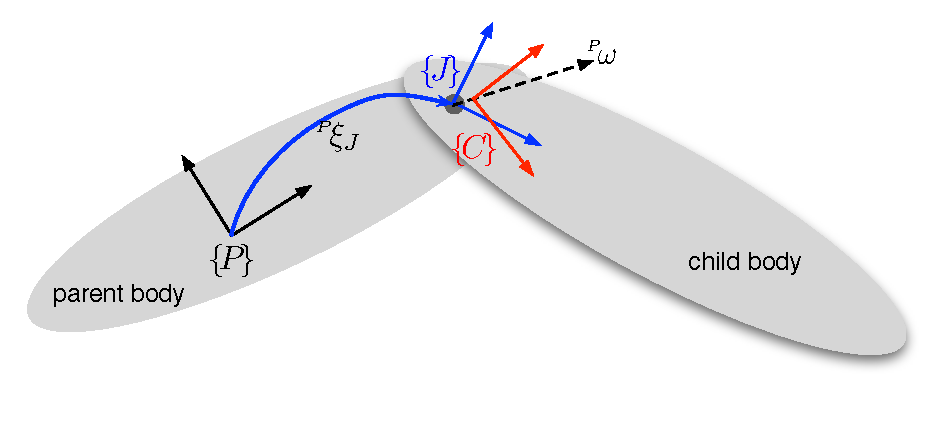
\includegraphics[width=0.8\textwidth]{frames}\\
\end{centering}
 \caption{Relationship between parent and child rigid bodies connected by a joint.}
 \label{fig:frames}
\end{figure}

URDF explicitly separates links and joints which the Denavit-Hartenberg notation merges together.  It is also more general and
supports branching mechanisms, that is, a link could have multiple child links which can be used to represent a humanoid robot.
Note that some URDF models may not be expressible in Denavit-Hartenberg notation.  

A number of different joint types are defined:
\begin{description}
\item[revolute] a  joint that rotates about the specified axis and has a limited range specified by the upper and lower limits.
\item[continuous] a revolute joint that has no upper or lower limits.
\item[prismatic] a  joint that slides along the specified axis, and has a limited range specified by the upper or lower limits.
\item[fixed]  is not really a joint because it cannot move. All degrees of freedom are locked. This type of joint does not require the axis. \item[calibration]
\item[floating] allows motion for all 6 degrees of freedom.
\item[planar] allows motion in a plane perpendicular to the axis.
\end{description}

For prismatic and revolute types the motion limits are specified by nested
elements like
\begin{XML}
<limit lower="-0.5" upper="0.5" />
\end{XML}
where the limits are given in units of radians or metres for revolute for prismatic joints respectively.  If either of the
\xml{upper} or \xml{lower} limit is not specified, a limit, it defaults to zero.


\subsubsection{Link transformations}
We will use the notation of \cite{Corke17a} where $\pose[X]_Y$ represents rigid-body motion from frame $\cframe{X}$ to $\cframe{Y}$ and 
$\oplus$ represents rigid-body motion composition.  
For this problem we consider three coordinates frames: \cframe{P} of the parent link, \cframe{C} of the child link and \cframe{J} of the 
joint.
The transformation from the link frame of the parent frame to the link frame of the child is shown in Fig. \ref{fig:frames} and given by
\[
\pose[P]_C = \pose[P]_J \oplus \pose[J]_C(q, \vec[C]{\omega}, \sigma)
\]
The first transform is a constant set by the\xml{origin} tag of the joint element.
The second transform represents the action of the joint itself which is defined by a rotation about ($\sigma=0$), or translation along ($\sigma=1$), the vector $\vec[P]{\omega}$ by the joint variable $q$.

%%%%%%%%%%%%%%%%%%%%%%%%%%%%%%%%%%%%%%%%%%%%%%%%%%%%%%%%%%%
\subsection{Visual appearance}
URDF can also be used to describe graphical objects.  A very simple example\footnote{This example 1 from the ROS URDF tutorial.} of this is

\begin{XMLNum}
<?xml version="1.0"?>
<robot name="myfirst">

  <link name="base_link">
    <visual>
      <geometry>
        <cylinder length="0.6" radius="0.2"/>
      </geometry>
    </visual>
  </link>
</robot>
\end{XMLNum}
which defines a cylinder, with its axis parallel to the z-axis,  of length 0.6\unit{m} and radius of 0.2\unit{m} centred at the world origin. 
Substituting line 7 for
\begin{XML}
        <box size="1 2 3"/>
\end{XML}
would draw a box centred at the world origin of lengths 1, 2 and 3\unit{m} in the x-, y- and z-directions respectively.

By default the cylinder or box is drawn centred at the origin of the link coordinate frame.  It can be repositioned by introducing an
\xml{origin} element.  For example 
\begin{XML}
      <origin rpy="0 1.57075 0" xyz="0 0 -0.3"/>
\end{XML}
after line 8 (within the \xml{visual} element) will \emph{first} translate the cylinder by -0.3\unit{m} in the z-direction so its top is now at $z=0$ and
\emph{then} rotate it by $pi/2$ about the y-axis.

The object is drawn with a default color\footnote{Red in RViz, grey in MATLAB RST.} 
but we can change that by altering the material of the link.
This can be done adding
\begin{XML}
      <material rgba="0 0 0.8 1" />    
\end{XML}
below line 9.  The four numbers are red, green, blue in the range 0 to 1 and alpha (0 transparent, 1 opaque).
Alternatively 
\begin{XMLNum}
<?xml version="1.0"?>
<robot name="myfirst">

  <material name="blue">
    <color rgba="0 0 0.8 1"/>
  </material>

  <link name="link">
    <visual>
      <geometry>
        <cylinder length="0.6" radius="0.2"/>
      </geometry>
      <material name="blue" />
    </visual>
  </link>
</robot>
\end{XMLNum}
we can create a named material, lines 4--6, and then specify it for the link in line 14.


%%%%%%%%%%%%%%%%%%%%%%%%%%%%%%%%%%%%%%%%%%%%%%%%%%%%%%%%%%%
\subsection{Combining kinematics and appearance}
Now we will extend our kinematic model of the planar 2-link robot with simple visual models of the links.
The links will be drawn as long thin boxes, red and green respectively (somewhat like Fig 7.2b in \cite{Corke17a}).
The URDF file is now
\begin{XMLNum}
<?xml version="1.0"?>
<robot name="planar2">

  <material name="red">
    <color rgba="1 0 0 0.8" />
  </material>
  <material name="green">
    <color rgba="0 1 0 0.8" />
  </material>

  <link name="base_link" />
  <link name="link1">
    <visual>
      <geometry>
        <box size="1 0.1 0.1" />
      </geometry>
      <origin xyz="0.5 0 0" />
      <material name="red" />
    </visual>
  </link>
  <link name="link2">
    <visual>
      <geometry>
        <box size="1 0.1 0.1" />
      </geometry>
      <origin xyz="0.5 0 0" />
      <material name="green" />
    </visual>
  </link>
  <link name="end">
    <visual>
      <geometry>
        <cylinder radius = "0.05" length="0.2" />
      </geometry>
    </visual>
  </link>

  <joint name="q1" type="continuous">
    <parent link="base_link" />
    <child link="link1" />
    <axis xyz="0 0 1" />
  </joint>
  <joint name="q2" type="continuous">
    <parent link="link1" />
    <child link="link2" />
    <origin xyz="1 0 0" />
    <axis xyz="0 0 1" />
  </joint>
  <joint name="notajoint" type="fixed">
    <parent link="link2" />
    <child link="end" />
    <origin xyz="1 0 0" />
  </joint>

</robot>
\end{XMLNum}
where lines 38--55 are as before.
Lines 4--9 define two translucent materials called \xml{red} and \xml{green} respectively.
Link 1 now has a \xml{visual} element defined in lines 13--19.  
The geometry is a box of length 1\unit{m} in the x-direction and
by default the reference frame of the visual element is with respect to the reference frame of the link.
One end of the box should be at joint 1, at the origin, so we shift it by 0.5\unit{m} in the x-direction using an \xml{origin} element (line 17).
Finally, we set the color to red using a \xml{material} element (line 18).
Link 2 is similar.

\begin{figure}
\begin{centering}
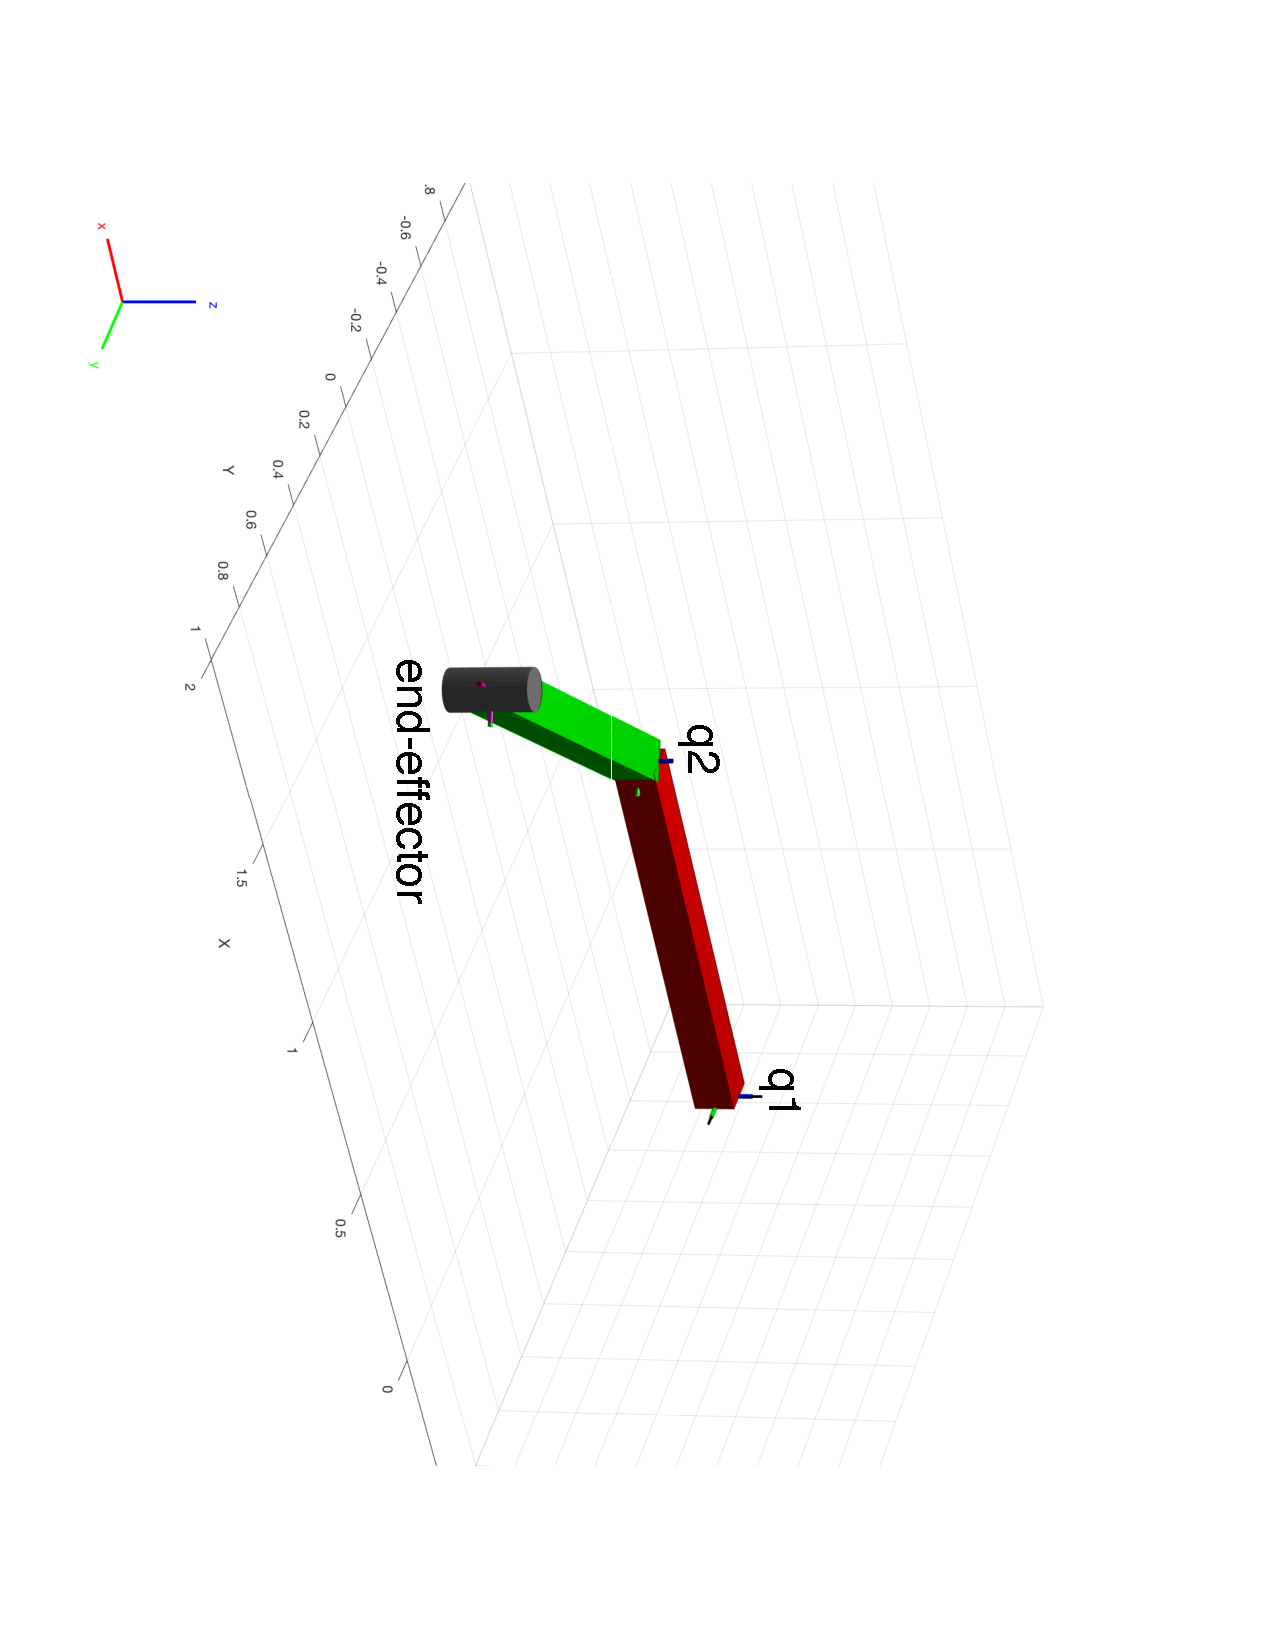
\includegraphics[angle=90,width=0.9\textwidth]{planar2.pdf}\\
\end{centering}
 \caption{Planar 2 robot with joint angles $[0, \pi/4]$ parsed and plotted using the Robotic Systems Toolbox\textsuperscript{\textregistered}.}
 \label{fig:planar2}
\end{figure}

The end of the robot is indicated by a small cylinder, in default color, which is centred at the origin of the end link's coordinate frame.

Using the Robotic Systems Toolbox\textsuperscript{\textregistered} the file can be parsed and displayed very simply by
\begin{Code}
>> r = importrobot('/Users/corkep/pic3.urdf')
>> r.DataFormat='row'
>> show(r, [0 pi/4])
\end{Code}
and the result is shown in Figure \ref{fig:planar2}.

%%%%%%%%%%%%%%%%%%%%%%%%%%%%%%%%%%%%%%%%%%%%%%%%%%%%%%%%%%%
\subsection{Displaying meshes}

The visual geometry can contain a \xml{mesh} element instead of \xml{cylinder} or \xml{box} as shown in this snippet\footnote{Exercepted from the Robotic Systems Toolbox file \texttt{iiwa14.urdf}.}
\begin{XMLNum}
    <visual>
      <origin rpy="0 0 0" xyz="0 0 0"/>
      <geometry>
        <mesh filename="package://iiwa_description/meshes/iiwa14/visual/link_6.stl"/>
      </geometry>
      <material name="Orange"/>
    </visual>
\end{XMLNum}
A \xml{mesh} element, line 4, specifies a a filename, and an optional scale factor that scales the mesh's axis-aligned-bounding-box. The recommended format for best texture and color support is Collada \texttt{.dae} files, though \texttt{.stl} files are also supported. The mesh file is not part of the URDF file and must be provided along with the URDF file and have the appropriate path.
The \xml{<mesh>} tag also supports a \xml{scale} option with a list of x-, y- and z-axis scale factors.

\begin{figure}
\begin{centering}
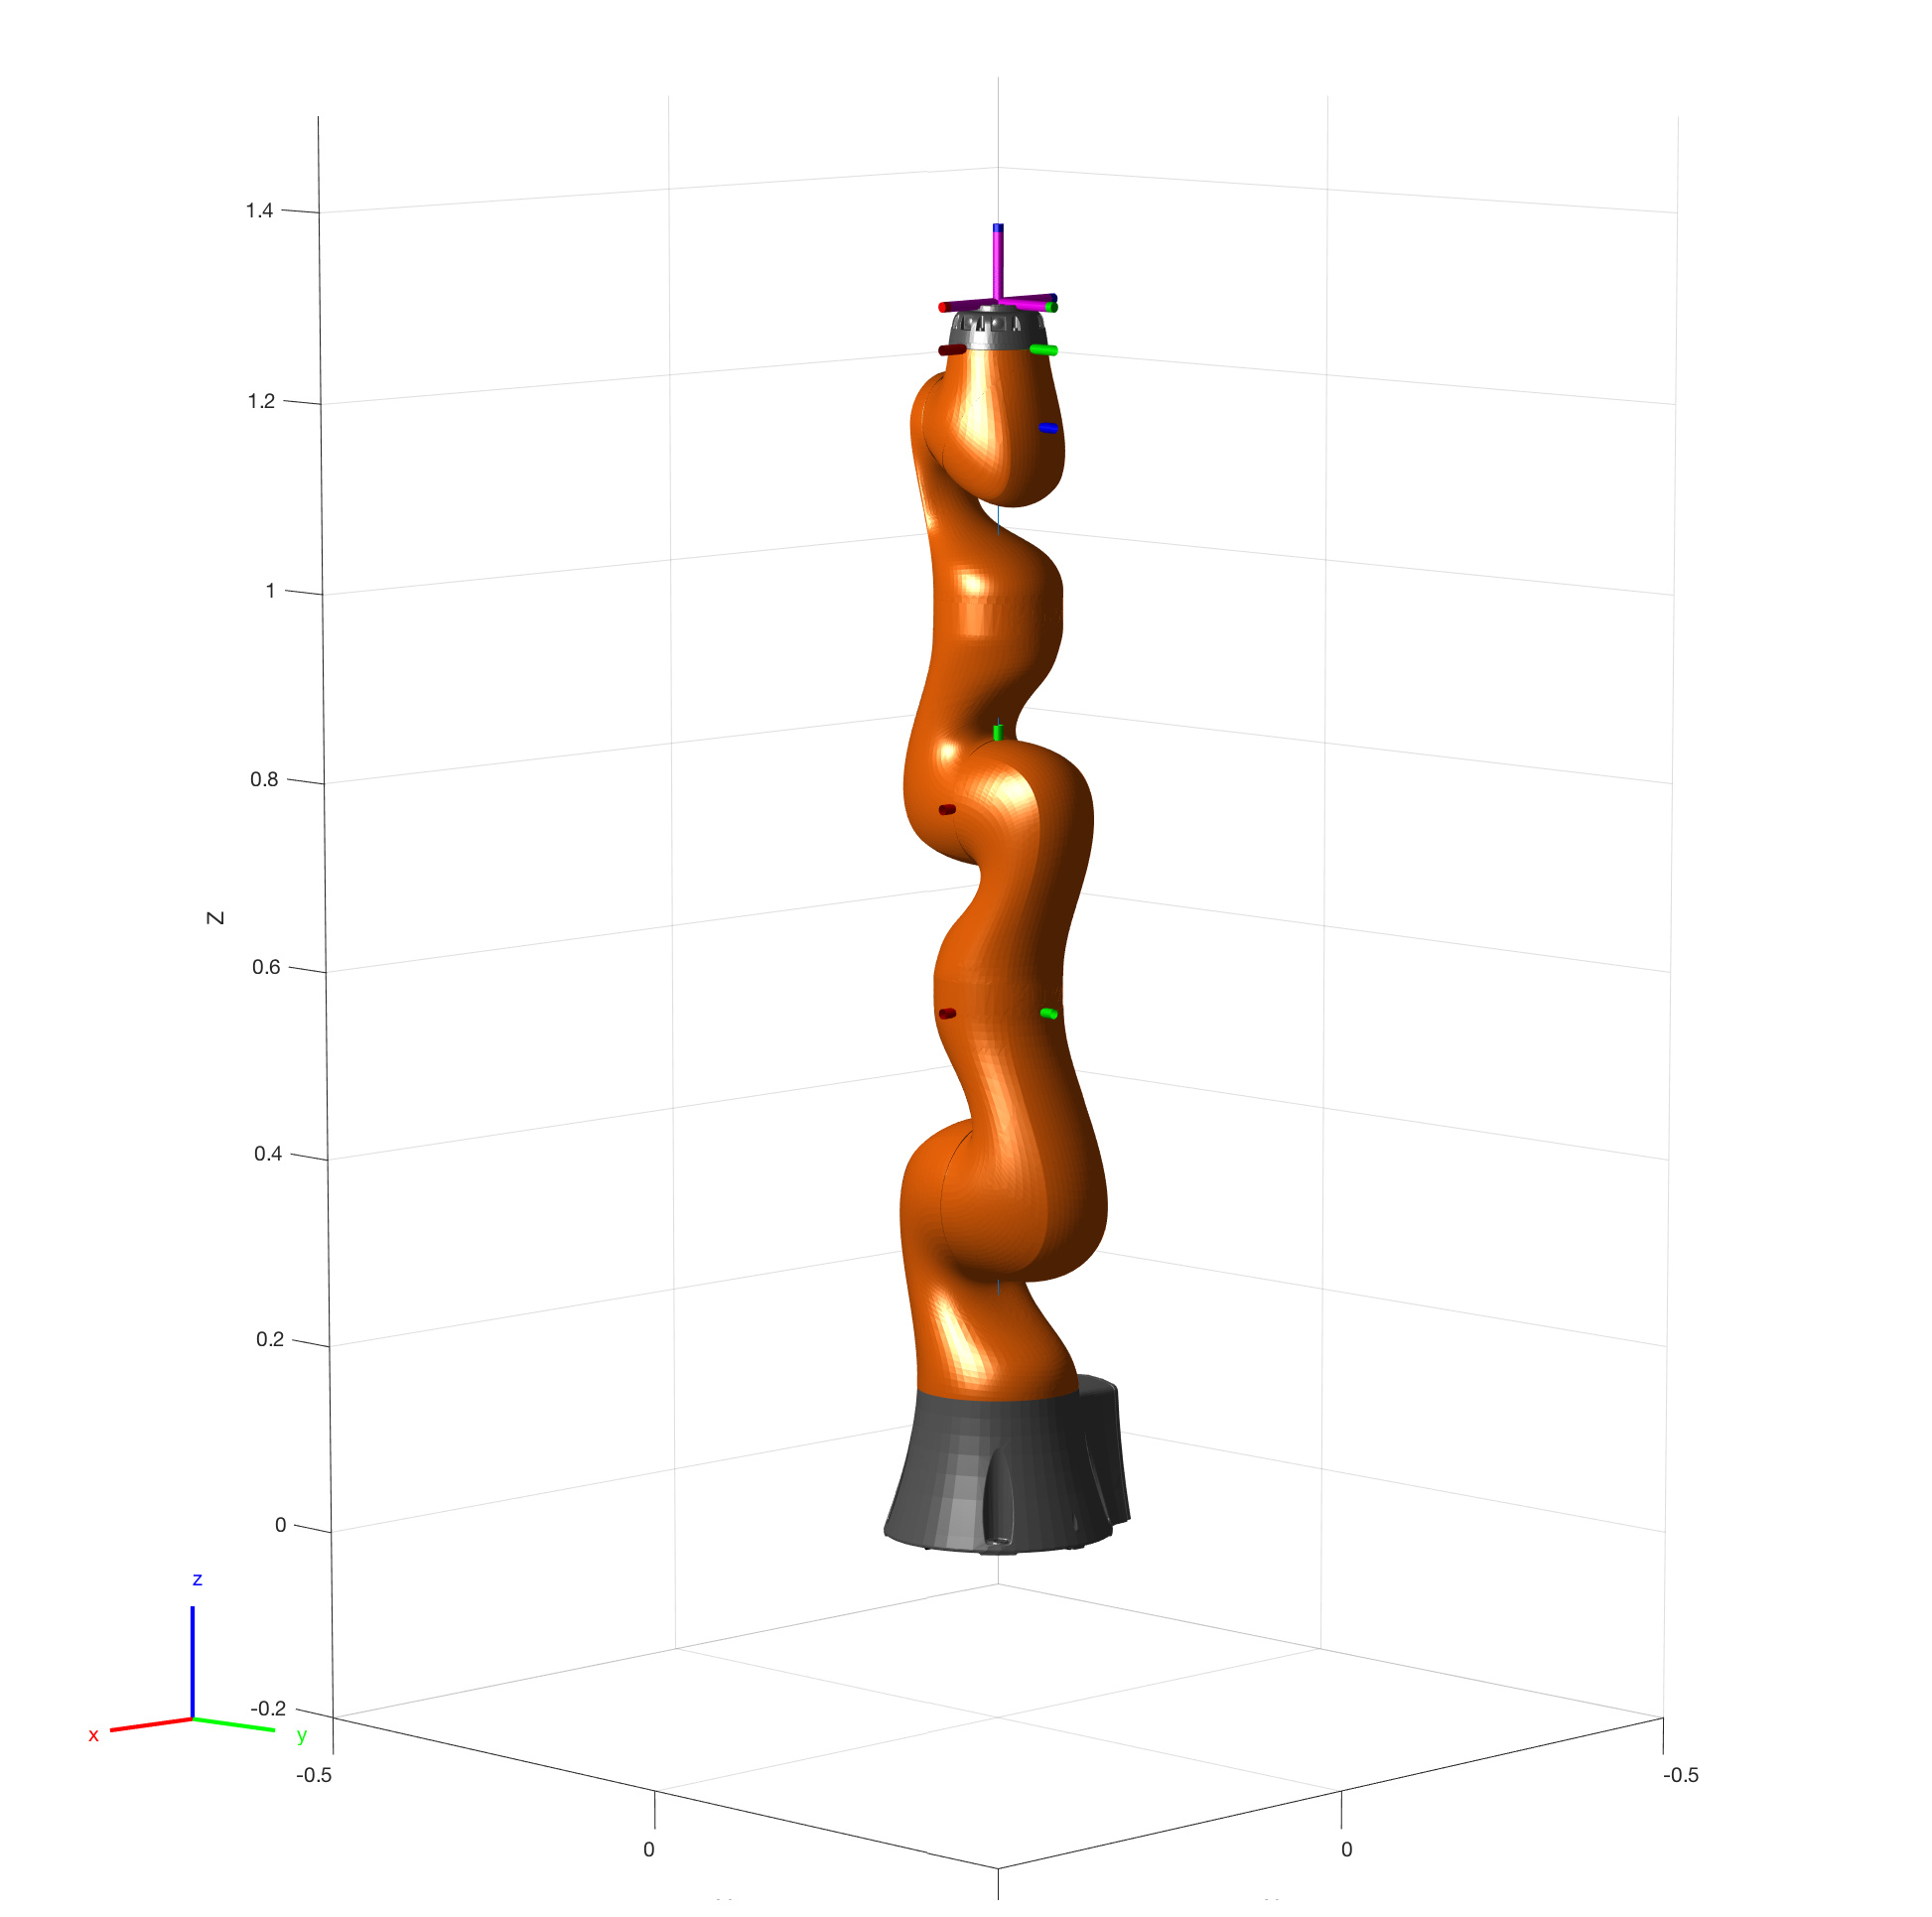
\includegraphics[width=0.8\textwidth]{iiwa}\\
\end{centering}
 \caption{Kuka iiwa14 robot.}
 \label{fig:iiwa}
\end{figure}

The Robotics System Toolbox includes a model of the Kuka iiwa14 arm and this can be imported, along with its meshes defined in STL
format, and displayed
\begin{Code}
>> robot = importrobot('iiwa14.urdf')
>> show(robot)
\end{Code}
and the result is shown in Figure \ref{fig:iiwa}.

%%%%%%%%%%%%%%%%%%%%%%%%%%%%%%%%%%%%%%%%%%%%%%%%%%%%%%%%%%%
\subsection{xacro macros}
Very large URDF files can be difficult to create and maintain, and this job can be simplified by introducing macros and even
conditional code.  The ROS package \texttt{xacro} is a macro-preprocessor written in Python that can be used to transform files written with
\texttt{xacro} macros into regular XML-based URDF which can be parsed as discussed above.
For example

\begin{Code}
<xacro:macro name="pr2_arm" params="suffix parent reflect">
  <pr2_upperarm suffix="${suffix}" reflect="${reflect}" parent="${parent}" />
  <pr2_forearm suffix="${suffix}" reflect="${reflect}" parent="elbow_flex_${suffix}" />
</xacro:macro>
<xacro:pr2_arm suffix="left" reflect="1" parent="torso" />
<xacro:pr2_arm suffix="right" reflect="-1" parent="torso" />
\end{Code}
expands to:
\begin{Code}
<pr2_upperarm suffix="left" reflect="1" parent="torso" />
<pr2_forearm suffix="left" reflect="1" parent="elbow_flex_left" />
<pr2_upperarm suffix="right" reflect="-1" parent="torso" />
<pr2_forearm suffix="right" reflect="-1" parent="elbow_flex_right" />
\end{Code}

It can also be useful for parameterizing elements
\begin{Code}
<xacro:property name="the_radius" value="2.1" />
<xacro:property name="the_length" value="4.5" />

<geometry type="cylinder" radius="${the_radius}" length="${the_length}" />
\end{Code}


\appendix
\section{A simple URDF parser in MATLAB}
Following is a fairly complete URDF parser that returns three structure arrays: \texttt{joints}, \texttt{links} and \texttt{materials}.
For the \texttt{links} array, the \texttt{material} field is an integer index into the \texttt{materials} array.
For the \texttt{joints} array, the \texttt{parent} and \texttt{child} fields are integer indices into the \texttt{links} array.
The source can be found in LiveScript file \texttt{urdfparse.mlx} and is for illustrative purposes only.
The Robotics Toolbox for MATLAB includes a complete parser as \texttt{urdfparse}.

\begin{Code}
root = xmlread(['planar2b.urdf']);

clear joints links materials

robot = root.getChildNodes.item(0);

materialNodes = robot.getElementsByTagName('material');
i = 1;
for j=1:materialNodes.getLength
    node = materialNodes.item(j-1);
    if isEqualNode(node.getParentNode, robot)
        % only process material nodes at the top level
        materials(i).name = string(node.getAttribute('name'));
        materials(i).rgba = str2num(node.getElementsByTagName('color').item(0).getAttribute('rgba'));
        materials(i).node = node;
        i = i + 1;
    end
end
try
    materialNames = [materials.name];
end

materialNames
\end{Code}
\begin{CodeGrey}
materialNames = 
    "red"    "green"
\end{CodeGrey}
\begin{Code}
materials(2)
\end{Code}
\begin{CodeGrey}
ans = 
    name: "green"
    rgba: [0 1 0 0.8000]
    node: [1x1 org.apache.xerces.dom.DeferredElementImpl]
\end{CodeGrey}
\begin{Code}

linkNodes = robot.getElementsByTagName('link');
for i=1:linkNodes.getLength
    node = linkNodes.item(i-1);
    links(i).name = string(node.getAttribute('name'));
    links(i).geometry = node.getElementsByTagName('geometry').item(0);
    try
        links(i).material = find(strcmp((node.getElementsByTagName('material').item(0).getAttribute('name')), materialNames));
    end

    try
        t = str2num( node.getElementsByTagName('origin').item(0).getAttribute('xyz'));
        rpy = str2num( node.getElementsByTagName('origin').item(0).getAttribute('rpy'));
    end
        if isempty(t)
            t = [0 0 0]; 
    end
    if isempty(rpy)
        rpy = [0 0 0];
    end
    links(i).T = SE3(t) * SE3.rpy(rpy);   
    links(i).node = node;
end

linkNames = [links.name]
\end{Code}
\begin{CodeGrey}
linkNames = 
    "base_link"    "link1"    "link2"    "end"
\end{CodeGrey}
\begin{Code}
links(2)
\end{Code}
\begin{CodeGrey}
ans = 
        name: "link1"
    geometry: [1x1 org.apache.xerces.dom.DeferredElementImpl]
           T: [1x1 SE3]
        node: [1x1 org.apache.xerces.dom.DeferredElementImpl]
    material: 1
\end{CodeGrey}
\begin{Code}

jointNodes = robot.getElementsByTagName('joint');
for i=1:jointNodes.getLength
    node = jointNodes.item(i-1);
    joints(i).name = string(node.getAttribute('name'));
    joints(i).type = string(node.getAttribute('type'));
    try
        joints(i).axis = node.getElementsByTagName('axis').item(0).getAttribute('xyz');
    end
    joints(i).parent = find(strcmp(node.getElementsByTagName('parent').item(0).getAttribute('link'), linkNames));
    joints(i).child = find(strcmp(node.getElementsByTagName('child').item(0).getAttribute('link'), linkNames));
    
    try
        t = str2num( node.getElementsByTagName('origin').item(0).getAttribute('xyz'));
        rpy = str2num( node.getElementsByTagName('origin').item(0).getAttribute('rpy'));
    end
    if isempty(t)
            t = [0 0 0]; 
    end
    if isempty(rpy)
        rpy = [0 0 0];
    end
    joints(i).T = SE3(t) * SE3.rpy(rpy);
    joints(i).node = node;
end

joints(2)
\end{Code}
\begin{CodeGrey}
ans = 
      name: "q2"
      type: "continuous"
      axis: [1x1 java.lang.String]
    parent: 2
     child: 3
         T: [1x1 SE3]
      node: [1x1 org.apache.xerces.dom.DeferredElementImpl]
\end{CodeGrey}


\bibliographystyle{IEEEtran}
\bibliography{strings,publist}
\end{document}
